\chapter{IMAGE DRIVEN MACHINE LEARNING METHODS FOR MICROSTRUCTURE RECOGNITION}
\label{chap:COMMAT}

\let\thefootnote\relax\footnotetext{
This chapter previously appeared as:
A. Chowdhury, E. Kautz, B. Yener, and D. Lewis. "Image driven machine learning methods for microstructure recognition."  \emph{Computational Materials Science}, vol. 123 pp. 176-187, 2016.}



%%% INTRODUCTION
\section{Introduction}
\label{intro}

This is the second chapter in the error reduction part of the Thesis. In this chapter, we attempt to minimize the classification error in the problem of microstructure characterization. In this chapter, we are optimizing the classification error by modifying multiple components of an image classification pipeline as a whole as shown in Fig. \ref{fig:chapter3}.

\begin{figure}[ht!]
\centering
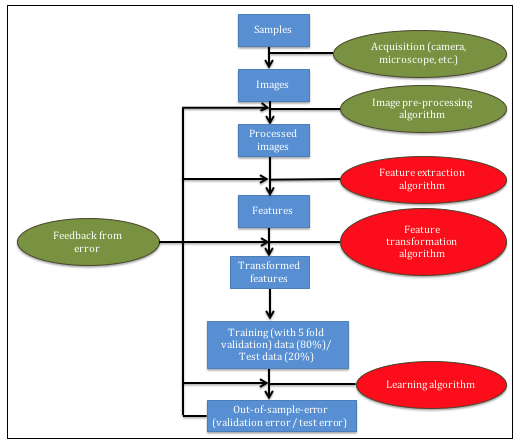
\includegraphics[width=1.0\textwidth]{img/chapter3}
\caption{Reducing classification error by optimizing the components of the image classification pipeline together instead of in isolation. The steps in the image classification pipeline highlighted in red are optimized simultaneously to minimize the classification error.}
\label{fig:chapter3}
\end{figure}

 Materials characterization is a critical aspect of the material design and discovery process.  Recently, there has been much research in the field of materials informatics, a growing research area in which information technology and data science methods are used to interpret and analyze material data in order to accelerate the material discovery, design, and development process \cite{XuH2015, Rodgers2006, Broderick2008, ferris2007materials, Kalidindi2011}.  Currently, material design relies on chance discoveries and follows a classical synThesis-characterization-theory-computation approach \cite{SergeiV.Kalinin2015}.  Further, there is a heavy reliance on individual researcher background and experience which introduces significant bias and potentially error into the process of microstructure recognition, interpretation, and characterization. 
%
For example, quantification of microstructures traditionally is done using stereological measurements.  Bias is introduced into stereological measurements through the requirement that an expert must first recognize and identify key microstructural features (inclusions, grains, or phases).  This bias can be caused by a variety of factors, such as an individual's background, education, and experiences \cite{SergeiV.Kalinin2015}.  

Although there have been recent advances in the field of quantitative microstructural science, there is still a heavy dependence on expert knowledge to identify what microstructural features are of interest for quantification \cite{DeCost2015}. Therefore it is desirable to expand upon work previously presented by DeCost and Holm in Reference \cite{DeCost2015}, and further explore methods of quantitative microstructure representations which do not require \textit{a priori} knowledge of microstructural features of interest or significance \cite{SergeiV.Kalinin2015}. This work aims to leverage existing computer vision and machine learning techniques specifically for the challenge of microstructure recognition.  While the overlap between computer vision, machine learning, and materials science is currently small \cite{SergeiV.Kalinin2015}, this work is a step towards increasing cross-disciplinary studies that challenge the current paradigm for microstructure characterization. 
%

Dendritic morphologies were chosen for this small case-study since dendrites are a well-characterized microstructural feature that exists in a variety of material systems (from single to multi-component).  Size, shape, and spacing of dendrites vary depending on solidification behavior and chemistry, thus micrographs of this single feature can vary widely.  The sample preparation and imaging methods used also contribute to the variety of micrographs produced from dendritic microstructures. Despite this variability in image data, it is still possible for human experts to look at a micrograph that contains dendrites and identify that it contains this microstructural feature, even though different orientations of dendrites (transverse or longitudinal) look distinctly different.  

Computer vision and machine learning methods were applied to the task of identifying a particular microstructural feature of interest (dendrites) from micrographs that do not contain this particular feature (just as a human expert would identify that a micrograph contains dendrites).  This recognition task is referred to in this work as Task 1.  Task 1 is high-level microstructure recognition in the sense that dendrites are a type of microstructural feature that are not specific to a material system.  A second classification task (referred to here as Task 2) was also completed, and involved distinguishing between longitudinal and transverse cross-sectional views of dendritic microstructures. This task may be viewed as a logical next step following the identification of dendrites in Task 1.

The contribution in this work is to investigate multiple computer vision and machine learning methods for microstructure recognition. We hypothesize that the approach and methods presented here can be generalized, and thus applied to a variety of microstructure recognition tasks that act as a necessary first step in characterization of a material system.
%-----------------------------------------

\section{Alloy Fabrication and Sample Preparation}
\label{sample_prep}

The alloy fabrication, processing, and metallographic sample preparation procedure followed to obtain images used in this work was based on the process detailed in References \cite{Schaefer2005} and \cite{Mao2014} and is summarized here. 
%

A Materials Research Furnaces (MRF) three probe arc melter was used to fabricate alloys of varying Sn-Ag-Cu compositions.  After melting, alloys were allowed to solidify and were then prepared for directional solidification (DS).  The solidified buttons were placed in a beaker on a hot plate.  The button was re-melted while constantly being purged with Ar gas to minimize sample oxidation. The alloy melt was then transferred into a 4 mm inner diameter quartz ampule with a mechanical pump.  The rods were allowed to cool, then removed from the ampule, and placed in a larger quartz ampule (5 mm inner diameter) for DS.  This ampule was then back-filled with Ar gas, sealed using a hydrogen torch, and inserted into the DS furnace.

DS was performed using a Bridgman-type apparatus in order to refine alloy microstructure.  The tube furnace in this apparatus is a Thermolyne Type-21100 fitted with an Omega temperature controller.
Following DS, alloys were removed from the quartz ampule, and small sections from the middle third of the rod were mounted in epoxy for metallographic sample preparation.  Sections were mounted such that transverse and longitudinal orientations of $\beta$-Sn dendrites could be viewed.  Samples were ground using silicon carbide (SiC) papers to 600 grit, then polished using 9, 3, and 1 $\mu$m diamond slurries.  Colloidal silica was used as the final polishing step and as a chemical etchant so that the dendritic microstructure would be readily visible using light optical microscopy.

%----------------------------------------------------------------------------------
\section{Image Data Sets}
\label{data_sets}

Image data used in this study includes micrographs taken over a span of approximately three years by students in the Lewis Research Group in the Materials Science and Engineering Department at Rensselaer Polytechnic Institute (RPI).  All images taken by Lewis Research Group members are of solder alloys with dendritic microstructures.  These alloys were manufactured, processed, and imaged at RPI, and a representative process of sample preparation was presented in Section \ref{sample_prep}.  In order to supplement micrographs obtained at RPI, micrographs from the publicly available Dissemination of Information Technology for the Promotion of Materials Science (DoITPoMS) library \cite{Barber2003} were used. Example images used in classification are provided in Figure \ref{fig:example_images}.   

Images were grouped into two data sets: Data Set 1 and Data Set 2, corresponding to classification Tasks 1 and 2 respectively. Data Set 1 is comprised of micrographs with and without dendritic morphologies.  This data set includes all images with dendrites (longitudinal and transverse cross-sections) from both the Lewis Group and the DoITPoMS micrograph library \cite{Barber2003}.  All micrographs that do not depict dendritic morphologies were obtained from the DoITPoMS library.  Data Set 1 includes 528 images that are each 227 by 227 square pixels. 264 original images were used in making Data Set 1 (132 micrographs containing dendrites and 132 micrographs without dendrites). Each original image is 270 by 500 pixels but includes a scale bar that interferes with feature extraction, therefore each image was cropped to yield two 227 by 227 square pixel images.  Thus, 528 images were used for classification. 

Data Set 2 is a subset of Data Set 1, and is comprised of micrographs that only contain dendrites, where each micrograph is either a transverse or longitudinal cross-sectional view.  Micrographs used in this data set include both images from the Lewis Group and the DoITPoMS micrograph library.  Data Set 2 contains a total of 188 images that are each 227 by 227 square pixels. As was done for Data Set 1, original images were cropped to remove the scale bar: 47 micrographs of each longitudinal and transverse sections (total of 94 original images) were cropped to create a 188 images used for classification.
%
\begin{figure}
  \begin{centering}
 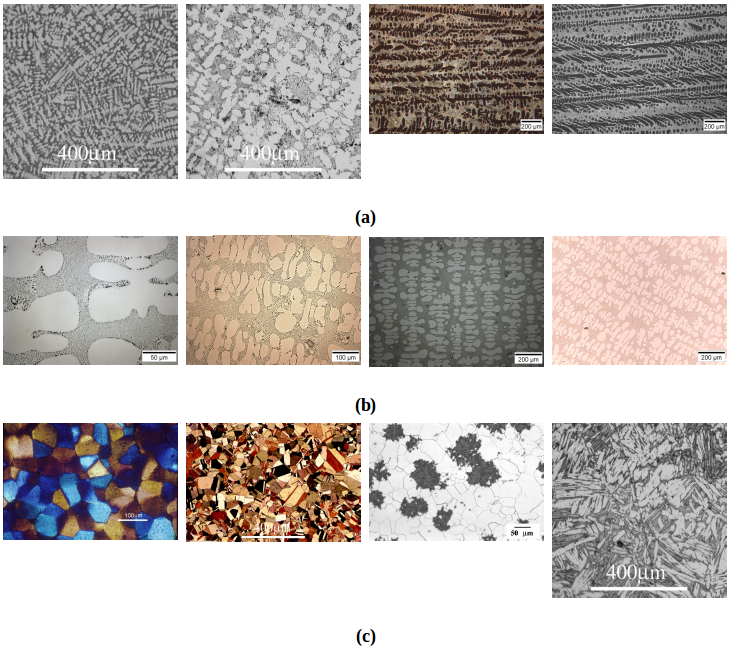
\includegraphics[scale=0.55]{img/example_images_v2.png}
 \caption{Examples of micrographs used in classification.  Micrographs shown in (a) and (b) are longitudinal and transverse cross-sectional views of dendrites, whereas micrographs in (c) do not contain dendrites.  Micrographs in (a), (b) and (c) were used in Task 1, and micrographs in (a) and (b) were used in Task 2.}
 \label{fig:example_images}
 \end{centering}
\end{figure}
%-----------------------------------------
\section{Approach}
\label{approach}
%
The general approach applied to the task of micrograph classification involved feature extraction and feature selection (dimensionality reduction) to compute feature vectors that were then used for training, validating, and testing various classification models.  The same approach was applied to both Data Sets 1 and 2 and is shown schematically in Figure \ref{fig:approach_overview}.

Feature extraction is the first step in the process of classifying micrographs.  Feature extraction starts with feature detection, where features in an image are local regions of pixels that include an `interesting' part of a microstructure, such as a corner, edge, or blob-like object. Features detected using computer vision algorithms are not necessarily semantically meaningful, however are pixel patterns that are mathematically repeatable and recognizable, thereby making the region a good feature. Detected features are then described (or represented) in the form of a vector, called a feature vector. A feature vector is comprised of a set of detected features in the image, and each image can thus be described or represented by a feature vector.  Multiple feature extraction methods were tested in this work in order to compare classification accuracies of different image representations.   
%

These feature vectors, derived in the process of feature extraction, have high dimensionality and in this work feature selection was performed after feature extraction for computational efficiency and to preclude the curse of dimensionality \footnote{The phrase `curse of dimensionality' refers to issues associated with increasing data dimensionality in Euclidean space.  Behavior of algorithms in low dimensional space, such as in three dimensions, may not generalize well to a higher dimensional space \cite{Keogh2010}.}.  Feature selection involves reducing the length of the feature vector while still retaining image information.  For example, if a feature vector is sparse, dimensionality reduction would involve reducing the sparsity of this vector.  Different dimensionality reduction methods were applied to test how each technique impacted classification accuracies.   

After feature extraction and selection, various classification models were trained, validated, and tested.  A 5 fold cross validation split was used for each data set.  This split was selected in order to minimize variance in model parameters%(determined via five-fold cross-validation on each of the 5 training folds), 
, and to avoid over-fitting.  These validation accuracies were then averaged and the standard deviation was calculated in order to evaluate model stability.  
%
\begin{figure}
  \begin{centering}
 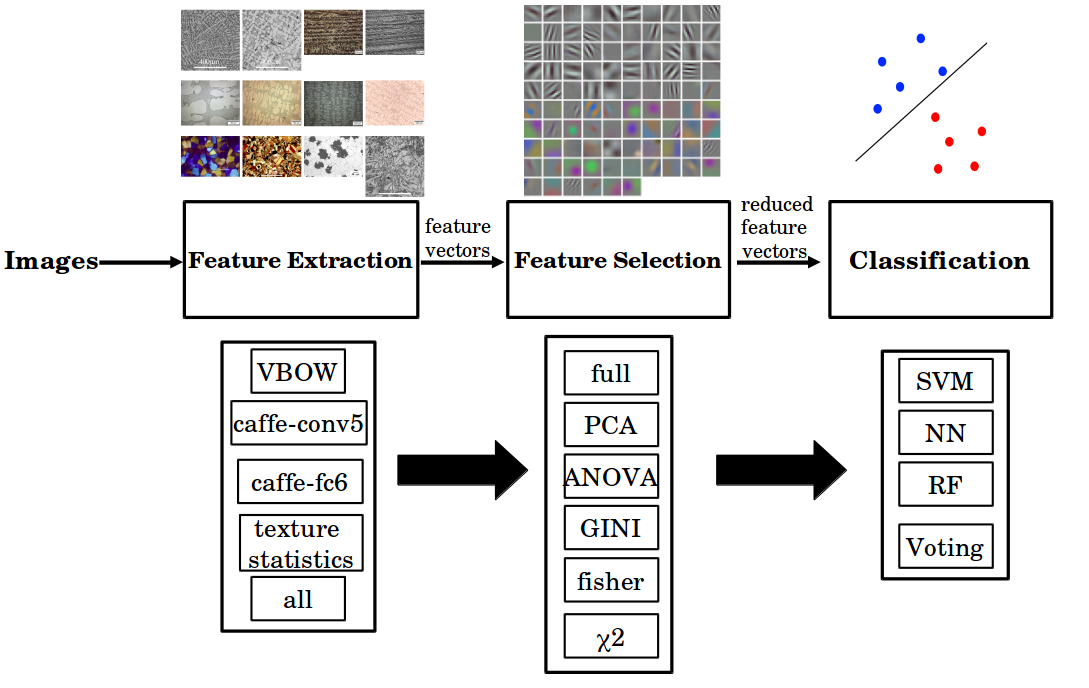
\includegraphics[scale=0.4]{img/flowchart_approach_updated.png}
 \caption{Overview of approach used in classification of micrograph data.  The approach summarized here shows 140 different combinations of feature extraction, feature selection and classification methods completed.  The same approach presented here was completed first for Task 1 (Data Set 1), then for Task 2 (Data Set 2).}
 \label{fig:approach_overview}
 \end{centering}
\end{figure}
%
We performed analysis on the two datasets (described in Section \ref{data_sets}) in the form of two classification tasks: Task 1 and Task 2. 

%The relationship between these tasks is depicted in Figure \ref{fig:tasks_flowchart}. 

%%Flowchart made using tikz
%\begin{figure}[t!]
%\centering
%\begin{adjustbox}{width=\textwidth,height=0.75\textheight,keepaspectratio}
%\subfigure[Task 1]{
%% \centering
%\begin{tikzpicture}
%[node distance =  5cm]
%    % Place nodes
%    \node [input] (input) {Input: Micrograph};
%    \node [decision, below of=input,yshift=-2cm] (task1) {Task 1: Does the micrograph depict a dendritic microstructure?};
%    % \node [decision, below of=task1,yshift=-2cm] (task2) {Task 2: Transverse cross-section?};
%    % \node [process, below of=task2,yshift=0cm] (trans) {Transverse cross-section of dendritic microstructure};
%    \node [process, below of=task1,yshift=0cm] (dendrite) {Dendritic microstructure};
%    \node [process, right of=task1, xshift=2cm] (nondendrite) {Non-dendritic microstructure};
%    % \node [process, right of=task2, xshift=4cm] (long) {Longitudinal cross-section of dendritic microstructure};
% 
%    % Draw edges
%   \path [line] (input) -- (task1);
%%   \path [line] (task1) -- node [anchor=east] {yes} (task2);
%  \path [line] (task1) -- node [anchor=east] {yes} (dendrite);
%   \path [line] (task1) -- node [anchor=south]{no} (nondendrite);
%%   \path [line] (task2) -- node [anchor=south]{no} (long);
%
%\end{tikzpicture}
%}
%
%\subfigure[Task 2]{
%% \centering
%\begin{tikzpicture}
%[node distance =  5cm]
%    % Place nodes
%    \node [input] (input) {Input: Dendritic Micrograph};
%    % \node [decision, below of=input,yshift=-1cm] (task1) {Task 1: Does the micrograph depict a dendritic microstructure?};
%    \node [decision, below of=input, yshift=-2cm] (task2) {Task 2: Transverse cross-section?};
%    \node [process, below of=task2,yshift=0cm] (trans) {Transverse cross-section of dendritic microstructure};
%    
%    % \node [process, right of=task1, xshift=4cm] (nondendrite) {Non-dendritic microstructure};
%    \node [process, right of=task2, xshift=2cm] (long) {Longitudinal cross-section of dendritic microstructure};
% 
%    % Draw edges
%   \path [line] (input) -- (task2);
%%   \path [line] (task1) -- node [anchor=east] {yes} (task2);
%   \path [line] (task2) -- node [anchor=east] {yes} (trans);
%%   \path [line] (task1) -- node [anchor=south]{no} (nondendrite);
%   \path [line] (task2) -- node [anchor=south]{no} (long);
%
%\end{tikzpicture}
%}
%\end{adjustbox}
%\caption{Flowchart of microstructure recognition tasks, referred to here as Task 1 and Task 2.  Tasks 1 and 2 are both binary classification tasks. (a) Task 1 involves distinguishing between micrographs that depict dendritic morphologies from those that do not contain this particular microstructural feature.  (b) Task 2 involves distinguishing between different cross-sectional views (longitudinal or transverse) of dendritic microstructures.}
%\label{fig:tasks_flowchart}
%\end{figure}
%----------------------------------------------------------------------------------
\section{Computer Vision and Machine Learning Methods}
\label{methods}

As previously introduced in Section \ref{approach}, multiple feature extraction and selection methods were tested with various classifiers in order to evaluate the best methods to apply to microstructure recognition tasks.  The methods applied in this work are discussed in additional detail in Sections \ref{feature_extraction} - \ref{classification}.  Additionally, Section \ref{related_work} provides a brief overview of computer vision and machine learning methods applied to other research in the field of materials science. 

\subsection{Feature extraction}
\label{feature_extraction}

Feature extraction methods applied in this work are texture and shape statistics (which include Haralick texture features \cite{Haralick1973}, histogram of oriented gradients (HoG) \cite{Dalal2005}, local binary patterns (LBP) \cite{Ojala2002}, Hu moments \cite{Hu1962,Otsu1975}, Zernike Moments \cite{Khotanzad1990},threshold adjacency statistics \cite{Lievers2004}), visual bag of words (VBOW) \cite{Yang2007,Bay2006}, and pre-trained convolutional neural networks (CNN's).  We used the publicly available Caffe framework \cite{Jia2014} for all experiments involving pre-trained CNN's. The network was based on the architecture of Krizhevsky \textit{et al.} for ImageNet \cite{Krizhevsky2012}.  The approach of using a pre-trained network was taken in this case-study because this is a good first step that does not require training to determine model parameters, which would be a difficult task with the small data sets used in this study \cite{Jia2014}. 
  
Texture and shape statistics involve multiple feature extraction algorithms (previously listed) that operate on image texture and shape of objects within the image.  These methods are introduced below:   

Haralick features \cite{Haralick1973} are calculated using gray-level co-occurrence matrices (\textit{G$_{ij}$}, shown below) which are square matrices of size \textit{N$_g$} x \textit{N$_g$}, where \textit{N$_g$} is the number of gray levels in an image:
\\
\begin{equation}
%\[
G_{ij}=
  \begin{bmatrix}
    p(1,1) & p(1,2) & \cdots       & p(1,N_{g}) \\
    p(2,1) & p(2,2) &  \cdots      & p(2,N_{g}) \\
     \vdots &  \vdots &  \ddots    &  \vdots          \\
    p(N_{g},1)  & p(N_{g},2) & \cdots & p(N_{g},N_{g}).
  \end{bmatrix}
%\]
\end{equation}
\\
Each matrix element, $ \ [i,j]\ $, is calculated by counting the number of times a pixel with value \textit{i} is adjacent to pixel with value \textit{j}.  When considering a square pixel image, there are four directions for which a gray-level co-occurrence matrix can be calculated: horizontal, vertical, left diagonal, and right diagonal.  Haralick texture statistics can be calculated based on the four gray-level co-occurrence matrices from each of these four directions. Haralick features thus describe the texture of an image. Fundamentally, texture is the arrangement of a certain feature or property, relative to the environment. In images, texture is the spatial distribution (arrangement) of gray-level variations in an image. Haralick features, computed from image gray-level co-occurrence matrices, capture texture patterns in an image. 

The histogram of oriented gradients (HoG) \cite{Dalal2005} method describes an image with a set of histograms of gradient orientations from local regions of an image (referred to as cells).  Each histogram reports the number of times a gradient orientation occurs in a given cell.  In general, an image gradient is a two-vector that points in the direction of the greatest rate of change.  The two components in the gradient vector include the gradient magnitude, $M(x,y)$, and the gradient orientation, $\alpha$$(x,y)$: 

\begin{equation}
%\[ M(x,y) = \sqrt{g_{x}^2+g_{y}^2} \]
M(x,y) = \sqrt{g_{x}^2+g_{y}^2}.
\end{equation}
%\\
\begin{equation}
%\[ \alpha(x,y) = \tan^{-1}({\frac{g_{x}}{g_{y}}})\]
\alpha(x,y) = \tan^{-1}({\frac{g_{y}}{g_{x}}}).
\end{equation}
\\
where $g_{x}$ and $g_{y}$ are the x and y components of the gradient respectively.  The normalized histograms of each cell are concatenated to form a descriptor vector for each image.  The greater the number of bins, the more detailed the histogram, and thus feature vector.

Local Binary Patterns (LBP) \cite{Ojala2002} method also describes the texture of an image.  Each image is split into cells and the neighborhood of each pixel (in each cell) is thresholded.  The neighborhood surrounding each pixel is defined by the pixel's eight nearest neighbors. When the center pixel intensity value is greater than its neighbor, the pixel value is changed to 0, otherwise the pixel value is 1. For each pixel, an 8-digit binary number, which can be referred to here as a label, is created. A histogram is created for each cell that reports the frequency of each label. The histograms for each cell are normalized, then all histograms are concatenated to yield a feature vector for the entire image. 

%A label is assigned by the operator to every pixel of an image by thresholding the neighborhood of each pixel with the center pixel value and using this result as a binary number. The local neighborhood is defined as a set of sampling points evenly spaced on a circle centered at the pixel to be labeled. Interpolation techniques are used when a sampling point does not fall on the center of the pixel.
%---------------------------------------------------------------------------------------------------------
Hu moments \cite{Hu1962,Otsu1975} are shape-based feature descriptors that describe, characterize, and quantify shapes of objects in an image.  
Hu moments are based on geometric moments, defined by $m_{p,q}(x,y)$: 

\begin{equation}
%\[ 
m_{p,q}(x,y) = \int_{-\infty}^{\infty} \int_{-\infty}^{\infty} x^{p} y^{q}f(x,y) dxdy.
%\].
\end{equation}
\\
Since images are a collection of pixels, the moment of an image must be expressed in terms of summations instead of integrals, as follows: 
\begin{equation}
%\[ 
m_{p,q}(x,y) = \sum_{-\infty}^{\infty} \sum_{-\infty}^{\infty} x^{p} y^{q}f(x,y) dxdy.
%\].
\end{equation}
\\

From the above equation, the area of an image would simply be defined by the 0th moment.  The centroid of an image can also be defined using this concept of geometric moments, as follows: 
\begin{equation}
%\[ 
(\bar{x},\bar{y}) = (\frac{m_{10}}{m_{00}} , \frac{m_{01}}{m_{00}}).  
%\].
\end{equation}
\\
When moments are taken with respect to an image centroid, the moments are translation invariant, therefore a geometric moment can be defined relative to the centroid by $\mu_{p,q}(x,y)$:  
\begin{equation}
%\[ 
\mu_{p,q}(x,y) = \sum_{-\infty}^{\infty} \sum_{-\infty}^{\infty} (x-\bar{x})^{p}(y-\bar{y})^{q}f(x,y)dxdy. 
%\]
\end{equation}
Hu derived seven moment invariants from the geometric moment equation, $\mu_{p,q}(x,y)$, that are invariant to scale, translation, and in-plane rotation and can be computed from a binary image. 
\\

In order to compute Hu moments, a binary image must be used.  A binary image was generated from the gray scale input images, by thresholding each image using Otsu's adaptive threshold algorithm \cite{Otsu1975}, which is a global thresholding method that selects the optimal threshold value based on the image histogram. Otsu's algorithm assumes the gray scale intensities of an image follow a bi-modal distribution with two classes, and the threshold value is selected to maximize the inter-class variance. Hu moments were computed based on connected components of pixels in the binary image.   \\

%-----------------------------------------
Zernike moments \cite{Khotanzad1990} are similar to Hu moments in that they describe the shape of objects in an image.  An important difference between Hu and Zernike moments is that Zernike polynomials are orthogonal basis functions for Zernike moments.  The use of orthogonal polynomials makes Zernike moments rotation invariant, and more robust to noise and minor variations in shape than Hu moments. Zernike moments are also calculated from a thresholded (binary) image.

%-----------------------------------------
Threshold adjacency statistics \cite{Lievers2004} are calculated from thresholded binary images. Three different binary images are generated from the original, using three different threshold values.  For each white pixel in an image, the number of neighboring white pixels is counted \cite{Klinger2012}.  The first statistic is the number of white pixels with no white neighbors.  The second statistic is the number of white pixels with one white neighbor.  The number of white pixels with white pixel neighbors up to eight is counted (where there are eight nearest neighbor for each pixel in an image).  Such statistics can be combined to create a feature vector that is subsequently used to distinguish and classify images.   

All texture and shape statistics used in feature extraction (Haralick texture features, HoG, LBP, Hu and Zernike moments, and threshold adjacency statistics) were used to create a 1,775 dimensional feature vector for each image that represents texture and shape of objects within the image. 

In addition to texture and shape statistics, Visual Bag of Words (VBOW), that was introduced in Chapter\ref{chap:ISBI} \cite{Yang2007,Bay2006} was also used for feature extraction. 
The VBOW technqiue is inspired from the  `bag of words' method used in document classification, where documents are considered as unordered sets of words. The corresponding words in the domain of image processing are local image features. These word descriptors are constructed around key points located by the Speeded Up Robust Features (SURF) \cite{Bay2006} key points detection algorithm.  These key points are extracted at regular locations at different scales making them very robust. The key point descriptors are categorized using a vector quantization technique such as $k$-means. The output of this discretization is a dictionary. Each image can therefore be encoded in the form of a histogram. This is done by extracting feature descriptors from the image, followed by finding the corresponding words to which the key points correspond to in the dictionary. The VBOW representation produced a 100-dimensional feature vector which was the pre-selected vocabulary size of the model.

A pre-trained convolutional neural network (CNN) model (trained on the Imagenet database) was also used in feature extraction. The ImageNet database contains 1.2 million images with 1000 categories. Here, the fifth and sixth layers of the pre-trained neural network were extracted and then used as feature descriptors for micrographs.
The sizes of the feature representation obtained from the pre-trained ImageNet model were 43,264 and 4,096 for the fifth layer (caffe-conv5) and sixth layer (caffe-fc6) respectively.  

Thus, for each image a feature vector was computed using each method described above. Concatenation of all computed feature vectors yielded a single vector which is referred to as \textgravedbl all\textacutedbl \ in Section \ref{results}.  Feature selection (dimensionality reduction) and classification was then performed using feature vectors from each method and the combined (concatenated) feature vector.     

\subsection{Dimensionality reduction}
\label{dimensionality_reduction}

Most of the image descriptors obtained from feature extraction methods lie in a high dimensional space (e.g. 1 x 43,264 for caffe-conv5).  Therefore it becomes necessary to employ dimensionality reduction techniques to bypass the curse of dimensionality \cite{curse}, and to improve computational efficiency.  The process of reducing feature vector dimensionality is called dimensionality reduction, or feature selection. Six different dimensionality reduction techniques were tested in this work: principle component analysis (PCA) \cite{pca}, ANOVA $F$-statistic (ANOVA) \cite{anova}, ${\chi}^2$ method \cite{chi}, Fisher score \cite{fisher}, and Gini index \cite{gini}. A brief description of each method is provided in this section. 

Principle component analysis (PCA)\cite{pca} is a feature transformation technique that uses orthogonal transformation to convert a set of observations of correlated variables to linearly uncorrelated ones. These orthogonal components are called principal components. In our work, we use only those principal components which account for 95 \% of the variance in the data. PCA can be thought of as a transformation that reveals the structure of the data in a way that best explains the variance in the data. The drawback of this technique is that the features obtained after reduction are linear combinations of the original feature variables which occupy a different vector space than the original variables. 

In addition to PCA, the Analysis of Variance (ANOVA) $F$-statistic \cite{anova} was used in feature selection. A one-way ANOVA F-test tests whether or not the different classes of the response variable have the same mean as the predictor variables. The $p$-value is calculated based on the $F$-statistic. These scores are then sorted in descending order and the features corresponding to the 30\textsuperscript{th} percentile are selected for analysis.

The ${\chi}^2$ test is used in statistics to test the independence of two events. In the domain of feature selection, it is used to test whether the occurrence of a particular variable and class are independent. The ${\chi}^2$ scores are ranked and the scores corresponding highest scores within the 30\textsuperscript{th} percentile are selected.

The idea behind the Fisher score is to find a subset of features such that the distance between data points in different classes is as large as possible and the distance between data instances in the same class are as small as possible. We select the features that correspond to the 30\textsuperscript{th} percentile of the highest Fisher scores.

%The idea behind the Minimum Redundancy Maximum Relevance (mrMR) \cite{mrmr} method was originally proposed by Pang et al. who proposed a feature selection technique that uses the mutual information criterion to score features. The key concept in  this feature selection procedure is to penalize a feature's relevancy by its redundancy in the presence of other selected features. The relevance of a feature subset is defined as the average value of the mutual information values between each individual feature and a particular class, whereas redundancy is the average of all the mutual information values between features. The mrMR criterion is therefore a combination of these two criteria (relevance and redundancy), which is defined as an optimization problem. The corresponding features which maximize the mrMR criterion are selected in this algorithm.

The Gini index \cite{gini} is an impurity splitting method, where impurity is calculated based on the probability that any sample belongs to a particular class. The minimum value of the index is 0, indicating that all of the members of the set belong to the same class, allowing for maximum useful information to be obtained. The opposite is true of samples in the set that are equally distributed in each class. The 30\textsuperscript{th} percentile threshold is used for selecting the features corresponding to Gini index scores.

\subsection{Classification}
\label{classification}

Classification was performed on Data Sets 1 and 2 using four different methods: support vector machine (SVM) \cite{svm}, random forest (RF)  \cite{rf}, nearest neighbor (NN)  \cite{nn}, and voting  \cite{voting}. SVM, NN, and Naive Bayes \cite{nb} models were used as components of the voting classifier.  Multiple classification algorithms were tested in order to determine which is the most accurate for micrograph classification. The classifiers applied to this case study were selected as representative models that have proven to yield high classification accuracies in other application areas, such as email filtering, text classification and more \cite{Kotsiantis2007}.  

Support vector machines (SVMs) \cite{svm} are discriminative (or margin based) classifiers. A SVM constructs a hyperplane in high dimensional space that may be used for classification. The hyperplane is selected such that the distance from it to the nearest data point on each side is maximized, referred to as the maximum margin hyperplane. We perform both linear and non-linear classification. We perform linear SVM classification on the original feature space and the non-linearity is introduced by the radial basis function (RBF) kernel for transforming data points to an infinite dimensional space. Our approach is to experiment with different learning algorithms. Therefore, we choose a representative algorithm from particular families of learning algorithms. The RBF kernel has proven to be a good representation for non-linear kernels. Linear SVM is referred to here as SVM-L, and non-linear SVM using a RBF is referred to as SVM-RBF.   

In addition to SVMs, nearest neighbor (NN) \cite{nn} classifier (an instance based classifier) was tested. The NN classifier assigns a test instance to a class based on the majority vote among the classes of the k-nearest neighbors of the training instances to the test instance. In our analysis, we selected k using five-fold cross validation. 

Random Forest (RF) classifiers \cite{rf}, also used in this work, are comprised of multiple decision trees and are therefore ensemble-based classifiers. A decision tree is a classification model that consists of a series of questions about the attributes of a data set, answers (such as yes or no), and follow-up questions. This series of questions is organized in a hierarchical manner and consists of edges that are connected to different types of nodes, including a root node, internal nodes, and leaf nodes. A root node has no incoming edges and zero or more outgoing edges.  An internal node has one incoming edge and two or more outgoing edges. A leaf node (also referred to as a terminal node) has one incoming edge and no outgoing edges. Each leaf node is assigned a label, and all internal and root nodes are assigned test conditions.  In order to perform classification using a decision tree model, a path is followed from root to terminal nodes.  This process will involve applying different test conditions, obtaining an answer, and moving to another internal node, and repeating this general process until a leaf/terminal node is reached.  The path followed in a decision tree model will yield a class label for a given data instance. Classification using RF is dependent on the prediction of class label from multiple decision trees. Each tree in the model gives a class label, and the RF chooses the class with the most votes among the decision trees. 
%-----------------------------------------
Similar to RF, the voting classifier \cite{voting} is also an ensemble-based classifier that is based on majority voting among various classification modules. With RF, the modules were decision trees, and in this work we perform voting among three independent algorithms: SVM-RBF, NN and Naive Bayes. \\

Naive Bayes is a classifier model that depends on the inherent distribution of the training data set, and is thus categorized as a generative classifier.  The Naive Bayes classifier uses Bayes' probability model and a decision rule to predict class of a data instance, where in this work each data instance is an image.    

%probability
Naive Bayes is a statistical classifier that uses the concept of posterior probability for classification of new data instances.  Each new data instance is assigned the class label that has the highest posterior probability. For a given set of variables $X={x_{1}, x_{2}, ..., x_{d}}$, the posterior probability for event $C_{j}$ is calculated from the set of possible outcomes, $C={c_{1}, c_{2}, ..., c_{d}}$, where the set of possible outcomes is all class labels. Bayes' rule defines posterior probability of a class label (the probability $X$ belongs to $C_{j}$) as:
%Bayes Rule 
\begin{equation}
p(C_{j}|x_{1}, x_{2}, ... x_{d}) \propto p(x_{1}, x_{2}, ...x_{d} | C_{j})p(C_{j}).
\end{equation}

where $p(C_{j}|x_{1}, x_{2}, ... , x_{d})$ is the posterior probability of class label $C_{j}$. Posterior probability can be re-written, given that conditional probabilities of independent variables are assumed to be statistically independent: 

\begin{equation}
p(C_{j}|X) \propto \prod_{k=1}^{d} p(C_{j}) p(x_{k}|C_{j}).
\end{equation}

Using the Naive Bayes classifier, the new data instance $X$ is classified by the class label $C_{j}$ that has the highest posterior probability. In addition to the probability model defined above, the maximum \textit{a posteriori} decision rule is applied for classification, meaning the hypoThesis that is most probable is selected as the class label.
%-----------------------------------------

Classification was completed using each of the methods detailed above, for the full data set in addition to the reduced data sets obtained by the different feature selection techniques detailed in Section \ref{dimensionality_reduction}.  Model parameters were determined using five-fold cross-validation.  

In order to determine model accuracy and stability, average classification accuracies and standard deviations were calculated for every possible combination of classification, feature extraction, and feature selection method used.  Average classification accuracies were calculated by taking the average of 5 fold cross validation of the dataset. The parameters of each algorithm were selected using the training fold of each split. Therefore the parameters were selected using another 5 fold cross validation of the training set and the training set was re-trained using the best combination of the parameters and the test accuracy on the remaining validation fold was calculated. This was performed 5 times and the average and standard deviation of the 5-fold validation accuracies was calculated.
%---------------------------------------------------------------------------------
%Methods that have been applied in the field of materials science and engineering....

\subsection{Related Work in Materials Science}
\label{related_work}

The methods discussed here are well established in the computer vision and machine learning disciplines, however only a select few have been previously applied to materials science and engineering challenges.  Shape descriptor methods, such as Hu moment invariants, have previously been used to quantitatively describe microstructures for subsequent classification \cite{Pattan2010, Prakash2011, Kumara,MacSleyne2008,Sluytman2012}.  
%
Specific applications of Hu moments in the field of materials science include automated classification of precipitate shapes in a two-phase microstructure \cite{MacSleyne2008}, classification of cast iron microstructures \cite{Pattan2010,Prakash2011,Kumara}, and analysis of precipitate shapes in nickel-based superalloys \cite{Sluytman2012}.\\

%
Additionally, the Visual Bag of Words feature extraction method with a Support Vector Machine classifier were used for multi-class classification of microstructures by DeCost and Holm \cite{DeCost2015}, as previously mentioned in Section \ref{intro}. 

%----------------------------------------------------------------------------------------------------------------------------
\section{Selection of Model Parameters}
Each algorithm involved in our experimentation has their own set of parameters. Some of the parameters are set \textit{a priori} and some are tuned using 5-fold cross-validation. Since we used cross validation to set the parameters for each combination of feature extraction, feature selection and classifier, there is no specific setting for each individual parameter for the algorithm. This approach of using 5-fold cross-validation to set parameters generates results that are more robust and thus more accurate with respect to each particular combination of feature extraction, feature selection, and classifier. We do a grid search over the parameter space using 5-fold cross-validation to estimate the best setting of the different parameters. Such parameters include number of neighbors in the nearest neighbor classifier, the SVM margin parameter ($C$), the RBF kernel parameter  ($\gamma$), the number of trees or estimators in the random forests classifier. The parameters found by cross-validation are presented in detail in the supplementary article to this chapter.

We also set a number of parameters before the experiments are run to limit the number of parameters to tune using cross-validation. 

%The Hessian threshold for the SURF detector was set to 500. The dictionary size for Visual Bag of Words was set to 100. The radius of the local binary patterns was set to 5 and the number of points to 10. The radius for Zernike moments was set to 5. 

%\begin{table}[H]
%\centering
%%\renewcommand{\arraystretch}{1}
%\captionsetup{justification=centering}
%\caption{Feature extraction parameters selected for use in experimentation.}
%\label{tab:parameters}
%%\resizebox{\linewidth}{!}{
%\begin{tabular}{|c|c|} \hline
%
%\textbf{Parameter}	&	\textbf{Value}	\\	\hline
%Hessian threshold for SURF detector & 500 \\ \hline
%Dictionary size for VBOW & 100 \\ \hline
%Radius of LBP & 5\\ \hline
%Number of points in LBP & 10 \\ \hline 
%Radius for Zernike moments & 5 \\ \hine
%\hline
%\end{tabular}
%%}
%\end{table}


Default values were used for other parameters. We set the parameters in the feature extraction algorithms because this would represent a consistent test bed for the thorough computational experimentation over the feature selection and classification algorithms.

\section{Software and Hardware Specifications}
All of our experimentation was carried out with Python version 2.7 with the help  of various open-source libraries. The opencv, scipy, skimage, numpy, mahotas and caffe packages (compatible with the Python version used in this work) were used for feature extraction. The skfeature library was used for experimentation with the various feature selection algorithms. The sklearn package was used for the various learning algorithms.

The hardware used for experimentation was a 3.3 GHz 4 core Intel i5 CPU.
%----------------------------------------------------------------------------------
\section{Results and Discussion}
\label{results}

This Section reports the results from applying multiple feature extraction, feature selection, and classification methods to the task of micrograph recognition.    
%
Performance comparisons between feature extraction, selection, and classification methods are presented in Sections \ref{Task1} and \ref{Task2}.  The success of different methods are compared based on the mean classification accuracies and standard deviations.
%
Results are presented in the form of tables, where each table compares all possible combinations of the three modalities (i.e. feature extraction, feature selection, and classification) that yield the maximum classification accuracy.  The tables presented here summarize a large set of results that are provided in a supplement to this article. 

%--------------------------------------------------------------
\subsection{Task 1 - Dendritic versus non-dendritic microstructures}
\label{Task1}

Table \ref{tab:FE_Task1} reports the feature extraction methods that yielded maximum classification accuracies for each combination of feature selection and classifier tested.  It is clear from Table \ref{tab:FE_Task1} that caffe-fc6 was the most effective feature extraction method because the majority of the maximum classification accuracies in Table \ref{tab:FE_Task1} were computed using feature vectors obtained using caffe-fc6.  These results suggest that microstructure image data is represented well using pre-trained neural networks (a type of deep learning algorithm), and this feature extraction method generalizes well.  

It is also important to note that caffe-fc6 was not re-trained on Data Sets 1 and 2 used in this case study.  The pre-trained weights determined via training on the millions of natural images in the ImageNet database were used, which were successfully applied to feature extraction here.  This result is significant because in using a pre-trained neural network, no large database (i.e. millions) of micrographs was needed.  The use of the sixth  layer (fully connected) from the Caffe network \cite{Jia2014} for feature extraction (caffe-fc6) resulted in superior classification performance over other feature extraction methods such as VBOW and texture and shape statistics for Task 1. 

It is suggested that caffe-fc6 produced higher classification accuracies overall than VBOW and texture and shape statistics for Task 1 based on the difference in image representations (in the form of feature vectors) between each method.  
%
Furthermore, caffe-fc6 provided a more accurate image representation than caffe-conv5 (the 5th convolution layer of the Caffe network).  This result could be due to the fact that features extracted from the sixth layer  was more representative of the image dataset. 

%--------------------------------------------------
%updated 06/10/16
\begin{table}[H]
\centering
\renewcommand{\arraystretch}{1}
\captionsetup{justification=centering}
\caption{Feature extraction methods and corresponding classification accuracies (in \%), that contributed to the maximum classification accuracy for each combination of feature selection and classification method tested for Task 1.}
\label{tab:FE_Task1}
\resizebox{\linewidth}{!}{
\begin{tabular}{|c|c|c|c|c|c|} \hline
	 & 	\multicolumn{5}{|c|}{\textbf{Classifier}} 									\\	\hline
\textbf{Feature }	&		&		&		&		&		\\	
\textbf{Selection}	&	\textbf{SVM-L}	&	\textbf{SVM-RBF}	&	\textbf{NN}	&	\textbf{RF}	&	\textbf{Voting}	\\	\hline
\multirow{2}{*}{\textbf{Full}}	&	\textbf{caffe-fc6}	&	\textbf{caffe-fc6}	&	\textbf{caffe-fc6}	&	\textbf{caffe-fc6}	&	\textbf{caffe-fc6}	\\	
	&	90.52 $\pm$ 4.9	&	90.52 $\pm$ 4.9	&	 87.69 $\pm$ 4.69	&	87.88 $\pm$ 6.19	&	89.02 $\pm$ 5.54	\\	\hline
\multirow{2}{*}{\textbf{PCA}}	&	\textbf{caffe-fc6}	&	\textbf{caffe-fc6}	&	\textbf{caffe-fc6}	&	VBOW 	&	\textbf{caffe-fc6}	\\	
	&	89.03 $\pm$ 3.58	&	89.03 $\pm$ 3.58	&	89.96 $\pm$ 2.53	&	87.88 $\pm$ 1.84	&	88.64 $\pm$ 3.09	\\	\hline
\multirow{2}{*}{\textbf{ANOVA}}	&	\textbf{caffe-fc6}	&	\textbf{caffe-fc6}	&	\textbf{caffe-fc6}	&	\textbf{caffe-fc6}	&	\textbf{caffe-fc6}	\\	
	&	90.91 $\pm$ 4.32	&	90.91 $\pm$ 4.32	&	87.31 $\pm$ 3.23	&	87.13 $\pm$ 5.35	&	91.85 $\pm$ 4.25	\\	\hline
\multirow{2}{*}{$\mathbf{{\chi}^2}$}	&	\textbf{caffe-fc6}	&	\textbf{caffe-fc6}	&	\textbf{caffe-fc6}	&	caffe-conv5 	&	\textbf{caffe-fc6}	\\	
	&	90.54 $\pm$ 3.99	&	 90.54 $\pm$ 3.99	&	87.3 $\pm$ 3.73	&	87.49 $\pm$ 4.5	&	90.53 $\pm$ 4.96	\\	\hline
\multirow{2}{*}{\textbf{fisher}}	&	\textbf{caffe-fc6}	&	\textbf{caffe-fc6}	&	\textbf{caffe-fc6}	&	texture-statistics 	&	texture-statistics 	\\	
	&	89.01 $\pm$ 5.82	&	 89.01 $\pm$ 5.82	&	89.58 $\pm$ 5	&	87.5 $\pm$ 6.1	&	89.58 $\pm$ 5.76	\\	\hline
\multirow{2}{*}{\textbf{GINI}}	&	texture-statistics 	&	texture-statistics 	&	\textbf{caffe-fc6}	&	texture-statistics 	&	caffe-conv5 	\\	
	&	89.01 $\pm$ 4.05	&	89.01 $\pm$ 4.05	&	89.39 $\pm$ 4.64	&	87.5 $\pm$ 5.46	&	89.58 $\pm$ 6.32	\\	\hline




\end{tabular}}
\end{table}
%----------------------------------------------------------------------------------

Feature selection was also investigated in order to determine if there was an overall best method for dimensionality reduction, and results are provided in Table \ref{tab:FS_Task1}.  From results presented here, there is no one feature selection method that provided maximum classification accuracies for the majority of feature extraction and classifier combinations tested.  This result could be attributed to the variability in the micrographs that do not depict dendrites (in Data Set 1).  The micrographs selected as depicting non-dendritic morphologies are not all from the same material system and there is no common microstructural feature amongst this class. 

The results also show that the feature selection method is sensitive to the types of feature extraction techniques and classifier models applied. Therefore, choice of dimensionality reduction should depend on the methods used for classification and feature extraction.

	
%-----------------------------------------------------------------------
%updated 06/09/16 - no mrmr in this table, no changes needed
\begin{table}[H]
\centering
\renewcommand{\arraystretch}{1}
\captionsetup{justification=centering}
\caption{Feature selection methods and corresponding classification accuracies (in \%), that contributed to the maximum classification accuracy for each combination of feature extraction and classification method tested for Task 1.}
\label{tab:FS_Task1}
\resizebox{\linewidth}{!}{
\begin{tabular}{|c|c|c|c|c|c|} \hline

	&	\multicolumn{5}{|c|}{\textbf{Classifier}} 									\\	\hline
\textbf{Feature }	&		&		&		&		&		\\	
\textbf{Extraction}	&	\textbf{SVM-L}	&	\textbf{SVM-RBF}	&	\textbf{NN}	&	\textbf{RF}	&	\textbf{Voting}	\\	\hline
\multirow{2}{*}{\textbf{VBOW}}	&	Full 	&	Full	&	Full	&	PCA	&	Full 	\\	
	&	86.93 $\pm$ 2.09	&	 86.93 $\pm$ 2.09	&	 84.45 $\pm$ 3.16	&	 87.88 $\pm$ 1.84	&	85.4 $\pm$ 3.53	\\	\hline
\multirow{2}{*}{\textbf{caffe-fc6}}	&	ANOVA 	&	ANOVA	&	PCA	&	Full	&	ANOVA	\\	
	&	90.91 $\pm$ 4.32	&	 90.91 $\pm$ 4.32	&	 89.96 $\pm$ 2.53	&	 87.88 $\pm$ 6.19	&	91.85 $\pm$ 4.25	\\	\hline
\multirow{2}{*}{\textbf{caffe-conv5}}	&	ANOVA 	&	ANOVA	&	ANOVA	&	${\chi}^2$	&	${\chi}^2$	\\	
	&	89.96 $\pm$ 6.11	&	89.96 $\pm$ 6.11	&	 85.04 $\pm$ 4.48	&	 87.49 $\pm$ 4.5	&	90.15 $\pm$ 5.08	\\	\hline
\multirow{2}{*}{\textbf{texture-statistics}}	&	${\chi}^2$	&	${\chi}^2$	&	fisher	&	fisher	&	${\chi}^2$	\\	
	&	 89.96 $\pm$ 5.37	&	89.96 $\pm$ 5.37	&	 89 $\pm$ 5.74	&	 87.5 $\pm$ 6.1	&	89.78 $\pm$ 4.82	\\	\hline
\multirow{2}{*}{\textbf{combined}}	&	${\chi}^2$	&	${\chi}^2$	&	fisher	&	GINI	&	${\chi}^2$	\\	
	&	89.96 $\pm$ 5.37	&	89.96 $\pm$ 5.37	&	 89 $\pm$ 5.74	&	86.74 $\pm$ 5.51	&	89.78 $\pm$ 4.8	\\	\hline

\end{tabular}}
\end{table}

%--------------------------------------------------------------------------------

Performance comparisons of classification models were also done for Task 1, and results are provided in Table \ref{tab:Classifier_Task1}.  Linear SVM (SVM-L) provides maximum classification accuracies for over 50\% of the possible feature extraction and selection combinations, indicating that this model generalizes well.
%%ARITRA- DOES THIS MAKE SENSE?: 
This result also demonstrates that the data is linearly separable and use of a Gaussian kernel is not necessary for Task 1. 

%--------------------------------------------------------------
%updated 06/10/16
\begin{table}[H]
\centering
\renewcommand{\arraystretch}{1}
\captionsetup{justification=centering}
\caption{Classification methods that contributed to the maximum classification accuracy (in \%) for each combination of feature extraction and feature selection method tested for Task 1.}
\label{tab:Classifier_Task1}
\resizebox{\linewidth}{!}{
\begin{tabular}{|c|c|c|c|c|c|} \hline
	&	\multicolumn{5}{|c|}{\textbf{Feature Extraction}} 									\\	\hline
\textbf{Feature }	&		&		&		&		&		\\	
\textbf{Selection}	&	\textbf{VBOW}	&	\textbf{caffe-fc6}	&	\textbf{caffe-conv5}	&	\textbf{texture-statistics}	&	\textbf{combined}	\\	\hline
\multirow{2}{*}{\textbf{Full}}	&	\textbf{SVM-L}	&	\textbf{SVM-L}	&	RF 	&	\textbf{SVM-L}	&	\textbf{SVM-L}	\\	
	&	 86.93 $\pm$ 2.09	&	90.52 $\pm$ 4.9	&	87.12 $\pm$ 4.37	&	 87.88 $\pm$ 3.98	&	 87.88 $\pm$ 3.98	\\	\hline
\multirow{2}{*}{\textbf{PCA}}	&	RF 	&	NN 	&	\textbf{SVM-L}	&	\textbf{SVM-L}	&	\textbf{SVM-L}	\\	
	&	87.88 $\pm$ 1.84	&	89.96 $\pm$ 2.53	&	87.3 $\pm$ 4.43	&	 88.64 $\pm$ 3.32	&	88.64 $\pm$ 3.32	\\	\hline
\multirow{2}{*}{\textbf{ANOVA}}	&	RF 	&	Voting	&	\textbf{SVM-L}	&	\textbf{SVM-L}	&	\textbf{SVM-L}	\\	
	&	83.72  $\pm$ 1.99	&	 91.85  $\pm$ 4.25	&	89.96  $\pm$ 6.11	&	89.78  $\pm$ 5.76	&	89.78  $\pm$ 5.76	\\	\hline
\multirow{2}{*}{$\mathbf{{\chi}^2}$}	&	\textbf{SVM-L}	&	\textbf{SVM-L}	&	Voting	&	\textbf{SVM-L}	&	\textbf{SVM-L}	\\	
	&	80.29 $\pm$ 3.58	&	90.54 $\pm$ 3.99	&	 90.15 $\pm$ 5.08	&	89.96 $\pm$ 5.37	&	89.96 $\pm$ 5.37	\\	\hline
\multirow{2}{*}{\textbf{fisher}}	&	\textbf{SVM-L}	&	NN 	&	Voting 	&	Voting	&	Voting	\\	
	&	78.4 $\pm$ 1.64	&	89.58 $\pm$ 5	&	89.57 $\pm$ 6.5	&	 89.58 $\pm$ 5.76	&	 89.58 $\pm$ 5.76	\\	\hline
\multirow{2}{*}{\textbf{GINI}}	&	Voting	&	NN	&	Voting	&	\textbf{SVM-L}	&	\textbf{SVM-L}	\\	
	&	 77.82 $\pm$ 2.85	&	 89.39 $\pm$ 4.64	&	 89.58 $\pm$ 6.32	&	 89.01 $\pm$ 4.05	&	 89.01 $\pm$ 4.05	\\	\hline

\end{tabular}}
\end{table}

The performance of the pipeline is also measured using the plot in Fig. \ref{fig:error_bars1}. Here, we sort the configurations in descending order based on the mean of their classification accuracies and plot the top 20 configurations with their corresponding error bars (one standard deviation).  We observe from this plot that there is a minor difference in the results with respect to top 20 configurations. However, we also observe that certain algorithms come up multiple times in the top 20 configurations. So, even though there isn't a clear \textit{best} configuration that is significantly better than all configurations, we can clearly see that there are certain algorithms which are better than others in terms of their ranking in the sorted order of configurations. We quantify this further by representing in Table \ref{table:average_rank1} the average rank of the algorithms with respect to their ranks in the sorted configurations. 
\begin{figure}[ht!]
  \begin{centering}
 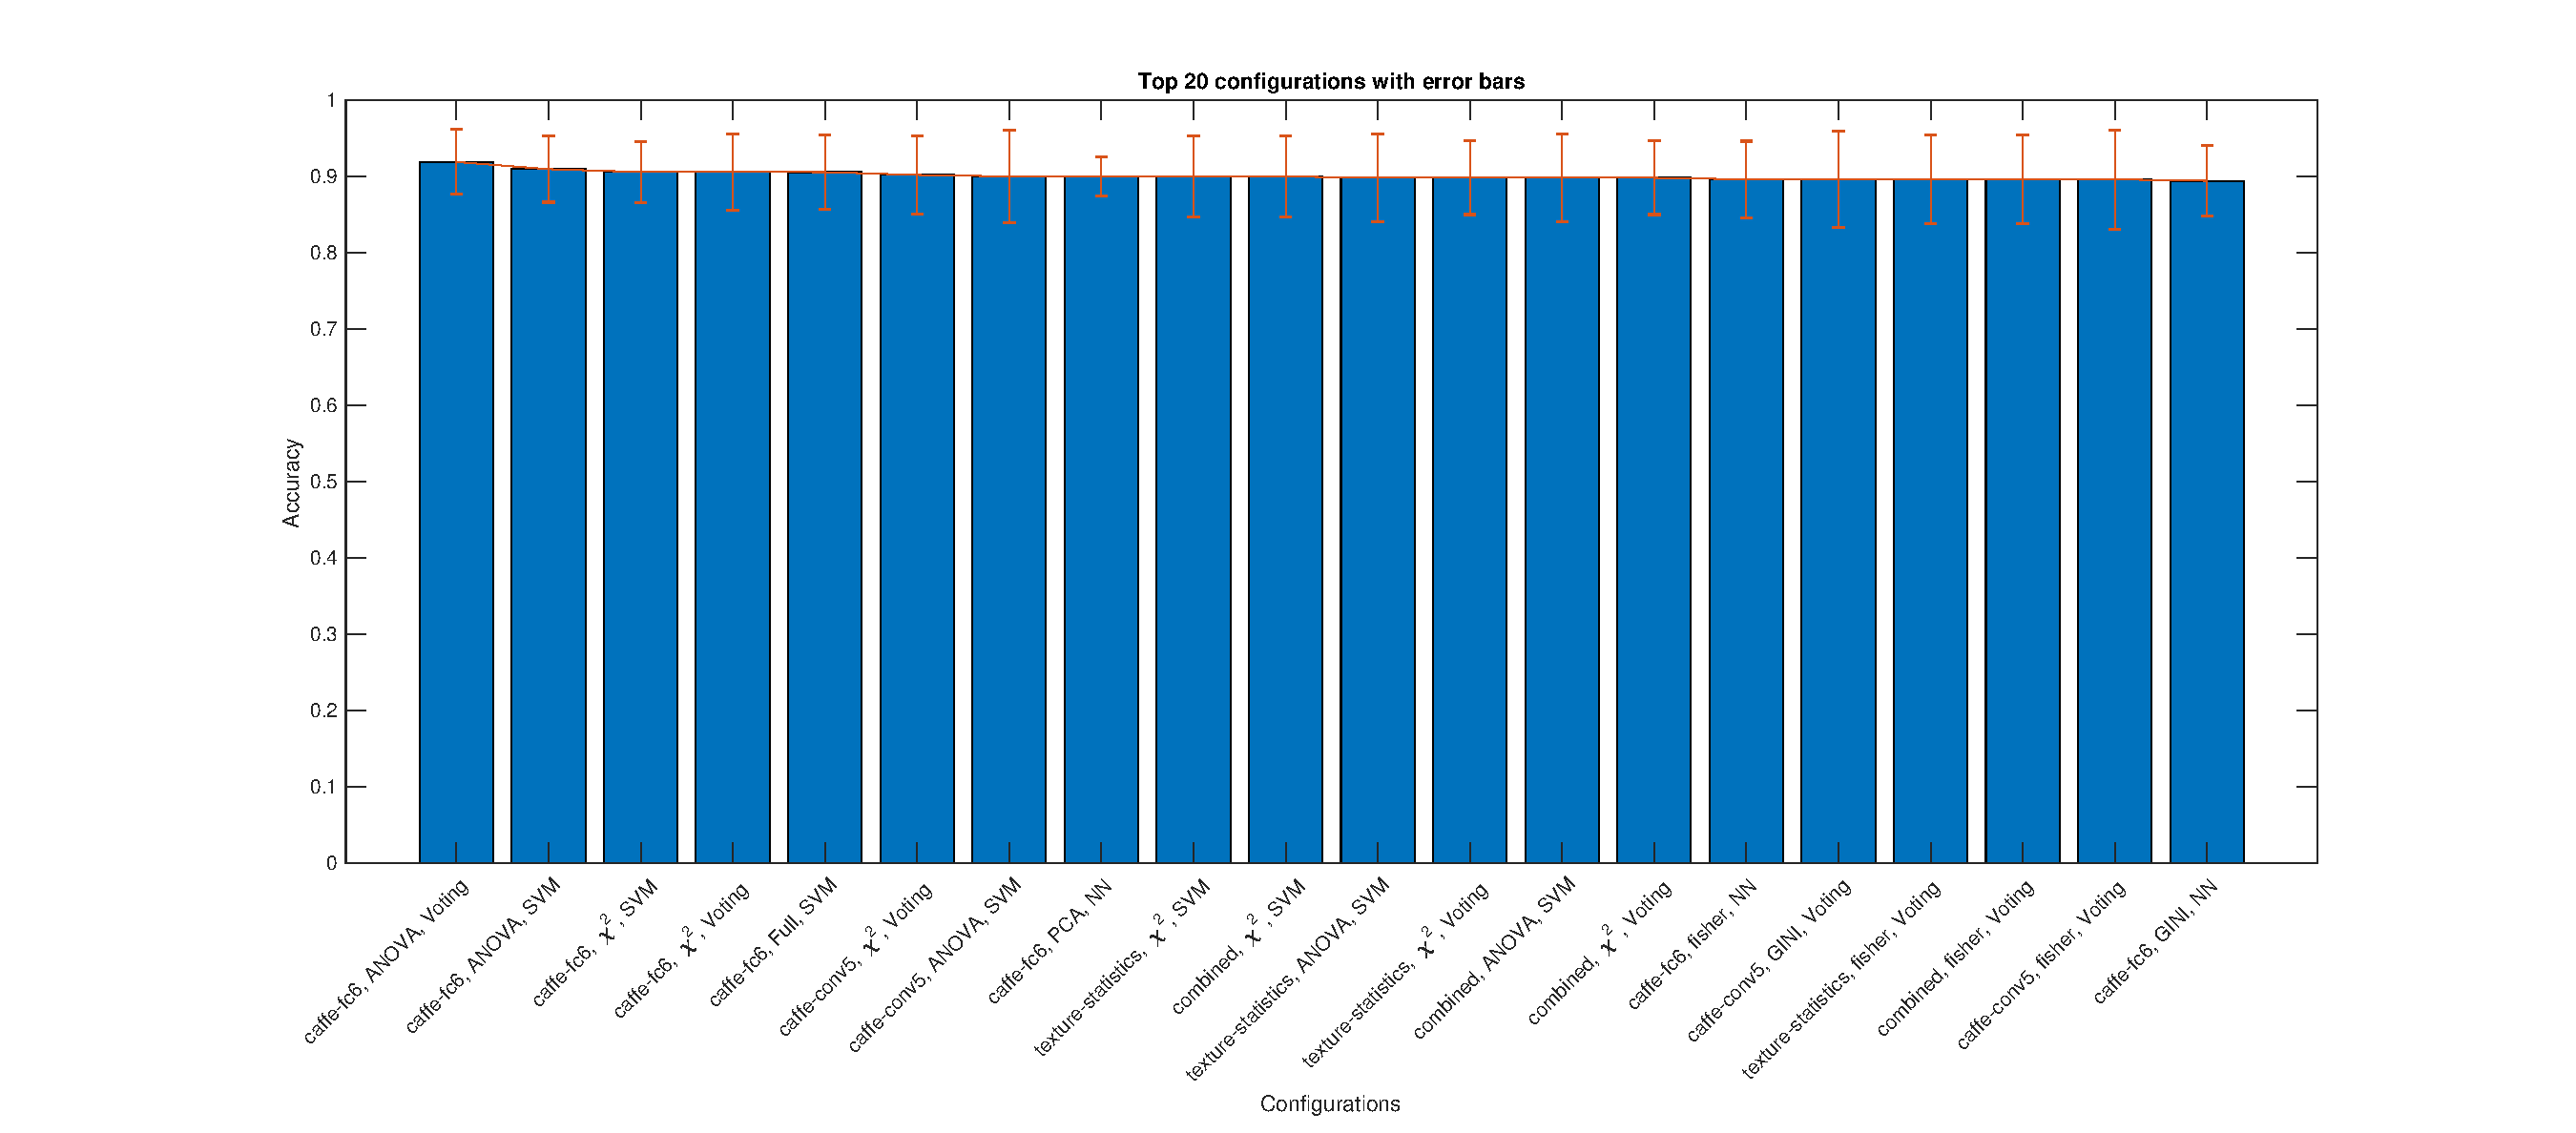
\includegraphics[scale=0.4]{img/best_matsc_error_bars_20.eps}
 \caption{Top 20 configurations of algorithms in Task 1 with error bars representing one standard deviation. There is no significant difference in the accuracies in the different configuations. Most of the feature extraction algorithms in the top 20 configurations are pre-trained CNNs (\textit{caffe-fc6} or \textit{caffe-conv5})}
 \label{fig:error_bars1}
 \end{centering}
\end{figure}

We can see from results in Table \ref{table:average_rank1} that caffe-fc6, $\chi^2$ and SVM are the best algorithms in the corresponding steps of feature extraction, dimensionality reduction and classification. However, caffe-fc6 has a larger margin with respect to the second best algorithm than $\chi^2$ and SVM in their respective steps. This indicates that caffe-fc6 is a good representation of the images for classification in Task 1.

\begin{table}[ht!]
\centering
\caption{Average rank of the algorithms in Task 1 with respect to feature extraction, dimensionality reduction and classification. The average rank of an algorithm quantifies it's position in the sorted list of configurations.}
\begin{tabular}{ |c|c| } 
 \hline
 \textbf{Feature extraction} & \textbf{Average rank} \\ 
 \hline
 \textbf{caffe-fc6} & \textbf{47.82}\\
 \hline
texture-statistics & 61.46\\
 \hline
combined& 64.46 \\
 \hline
caffe-conv5 & 72.39\\
 \hline
VBOW & 106.36\\
 \hline
 \hline
 \textbf{Dimensionality reduction} & \textbf{Average rank} \\ 
 \hline
 \textbf{$\chi^2$} & \textbf{54.45}\\
 \hline
fisher & 58.05\\
 \hline
PCA & 60.95 \\
 \hline
ANOVA & 61.80\\
 \hline
GINI & 66.10\\
 \hline
 Full & 66.55\\
 \hline
 \hline
 \textbf{Classification} & \textbf{Average rank} \\ 
 \hline
\textbf{SVM} & \textbf{54.57}\\
 \hline
Voting & 60.8\\
 \hline
RF & 81.40 \\
 \hline
NN & 85.23\\
 \hline
 \end{tabular}
\label{table:average_rank1}
\end{table}

%--------------------------------------------------------------
\subsection{Task 2 - Longitudinal versus transverse cross-sectional views of dendrites} 
\label{Task2}
%--------------------------------------------------------------

Similar performance comparisons presented for Task 1 in Section \ref{Task1} were also completed for Task 2 (longitudinal vs. transverse cross-sectional views of dendrites).  A similar result was observed when feature extraction methods were evaluated, where caffe-fc6 represented micrographs well. 

Again, features extracted using pre-trained neural networks dominates Table \ref{tab:FE_Task2}. This result shows that the features extracted from the sixth, fully connected layer in the Caffe network (caffe-fc6) have meaningful and distinguishable characteristics in terms of microstructural images.  
%
Although the majority of the maximum classification accuracies used features extracted via caffe-fc6, even higher values for classification accuracy were obtained using texture statistics and caffe-conv5 with a a linear SVM classifier. Classification accuracies obtained via SVM-L varied based on the feature selection method used, however the overall classification accuracies were highest for this classifier with features computed from either texture statistics or caffe-conv5.  %These feature extraction methods, used in conjunction with various feature selection techniques and SVM-L could have resulted in higher classification accuracies due to.........
%
One major disadvantage of using texture statistics for feature extraction is that this method is a combination of multiple different feature detectors, and required prior knowledge of various techniques, that all perform differently depending on shape and texture of input data. 
%
The success of SVM as a classifier is subsequently discussed in additional detail.  

%---------------------------------------------------------------
%updated 06/10/16 - mrMR removed
\begin{table}[ht!]
\centering
\renewcommand{\arraystretch}{1}
\captionsetup{justification=centering}
\caption{Feature extraction methods and corresponding classification accuracies (in \%), that contributed to the maximum classification accuracy for each combination of feature selection and classification method tested for Task 2.}
\label{tab:FE_Task2}
\resizebox{\linewidth}{!}{
\begin{tabular}{|c|c|c|c|c|c|} \hline
	 & 	\multicolumn{5}{|c|}{\textbf{Classifier}} 									\\	\hline
\textbf{Feature }	&		&		&		&		&		\\	
\textbf{Selection}	&	\textbf{SVM-L}	&	\textbf{SVM-RBF}	&	\textbf{NN}	&	\textbf{RF}	&	\textbf{Voting}	\\	\hline
\multirow{2}{*}{\textbf{Full}}	&	texture-statistics 	&	\multirow{14}{*}{\textbf{caffe-fc6:} 95.74 $\pm$ 3.73}	&	\multirow{14}{*}{\textbf{caffe-fc6:} 94.49 $\pm$ 1.46}	&	\textbf{caffe-fc6} 	&	\multirow{14}{*}{\textbf{caffe-fc6:} 94.99 $\pm$ 2.38 }	\\	
	&	95.79 $\pm$ 3.94	&		&		&	87.88 $\pm$ 1.64	&		\\	
\multirow{2}{*}{\textbf{PCA}}	&	texture-statistics 	&		&		&	VBOW 	&		\\	
	&	96.84 $\pm$ 3.07	&		&		&	87.88 $\pm$ 2.95	&		\\	
\multirow{2}{*}{\textbf{ANOVA}}	&	texture-statistics 	&		&		&	\textbf{caffe-fc6} 	&		\\	
	&	97.37 $\pm$ 3.33	&		&		&	87.13 $\pm$ 1.64	&		\\	
\multirow{2}{*}{$\mathbf{{\chi}^2}$}	&	caffe-conv5 	&		&		&	caffe-conv5 	&		\\	
	&	96.78 $\pm$ 2.63	&		&		&	87.49 $\pm$ 15.69	&		\\	
\multirow{2}{*}{\textbf{fisher}}	&	caffe-conv5 	&		&		&	texture-statistics 	&		\\	
	&	97.84 $\pm$ 2.65	&		&		&	87.5 $\pm$ 8.25	&		\\	
\multirow{2}{*}{\textbf{GINI}}	&	caffe-conv5 	&		&		&	texture-statistics 	&		\\	
	&	97.31 $\pm$ 2.42	&		&		&	87.5 $\pm$ 8.25	&		\\	\hline

\end{tabular}}
\end{table}

%----------------------------------------------------------------------------------
Results from comparing feature extraction and classifier combinations indicate that in many cases feature selection did not improve calculated classification accuracies, as was seen in Task 1 results.  This is shown in Table \ref{tab:FS_Task2} by the majority of maximum classification accuracies computed using the full feature vector. 
%
When SVM-L was used for classification, feature selection methods improved results.  The feature selection method used with SVM-L that yielded the maximum classification accuracy depended on the feature representation obtained in the feature extraction step. 
%
The same classification accuracies were obtained for each feature selection method, for a given feature extraction and classifier combination. In addition, the features extracted from the fifth layer (convolutional) in the pre-trained neural network perform poorly with respect to the other extraction methodologies. This can be attributed to the fact that caffe-conv5 produces the feature representation with the highest dimensionality which is an order of magnitude greater than the second largest feature vector (caffe-fc6). Therefore, features extracted using caffe-conv5 are not robust (i.e. they have low accuracy with high standard deviation).  Being lower in the network hierarchy of the CNN also means that the features may not be tuned properly to the task, and therefore features provide a less accurate image representation than features computed via caffe-fc6.  
%----------------------------------------------------------------------------------
\begin{table}[ht!]
\centering
\renewcommand{\arraystretch}{1}
\captionsetup{justification=centering}
\caption{Feature selection methods, and corresponding classification accuracies (in \%), that contributed to the maximum classification accuracy for each combination of feature extraction and classification method tested for Task 2.}
\label{tab:FS_Task2}
\resizebox{\linewidth}{!}{
\begin{tabular}{|c|c|c|c|c|c|} \hline
	&	\multicolumn{4}{|c|}{\textbf{Classifier}} 							\\	\hline		
\textbf{Feature }	&		&		&		&		&		\\	
\textbf{Extraction}	&	\textbf{SVM-L}	&	\textbf{SVM-RBF}	&	\textbf{NN}	&	\textbf{RF}	&	\textbf{Voting}	\\	\hline
\multirow{2}{*}{\textbf{VBOW}}	&	ANOVA 	&	\textbf{Full}	&	\textbf{Full}	&	PCA 	&	\textbf{Full}	\\	
	&	96.32 $\pm$ 2.68	&	93.73 $\pm$ 3.96	&	 92.73 $\pm$ 3.91	&	87.88 $\pm$ 2.95	&	93.98 $\pm$ 3.09	\\	\hline
\multirow{2}{*}{\textbf{caffe-fc6}}	&	GINI 	&	\textbf{Full}	&	\textbf{Full}	&	\textbf{Full}	&	\textbf{Full}	\\	
	&	96.78 $\pm$ 2.63	&	95.74 $\pm$ 3.73	&	94.49 $\pm$ 1.46	&	87.88 $\pm$ 1.64	&	94.99 $\pm$ 2.38	\\	\hline
\multirow{2}{*}{\textbf{caffe-conv5}}	&	fisher 	&	\textbf{Full}	&	\textbf{Full}	&	${\chi}^2$	&	\textbf{Full}	\\	
	&	97.84 $\pm$ 2.65	&	84.46 $\pm$ 13.6	&	77.19 $\pm$ 14.62	&	 87.49 $\pm$ 15.69	&	78.45 $\pm$ 16.66	\\	\hline
\multirow{2}{*}{\textbf{texture-statistics}}	&	ANOVA 	&	\textbf{Full}	&	\textbf{Full}	&	fisher 	&	\textbf{Full}	\\	
	&	97.37 $\pm$ 3.33	&	93.23 $\pm$ 11.58	&	94.24 $\pm$ 5.03	&	87.5 $\pm$ 8.25	&	93.73 $\pm$ 11.09	\\	\hline
\multirow{2}{*}{\textbf{combined}}	&	ANOVA 	&	\textbf{Full}	&	\textbf{Full}	&	GINI 	&	\textbf{Full}	\\	
	&	97.37 $\pm$ 3.33	&	89.97 $\pm$ 9.08	&	87.97 $\pm$ 9.02	&	86.74 $\pm$ 2.98	&	84.46 $\pm$ 14.08	\\	\hline

\end{tabular}}
\end{table}

%-------------------------------------------------------------------------------------

Lastly, classification models were evaluated for each combination of feature extraction and feature selection with results presented in Table \ref{tab:Classifier_Task2}. SVM-L provided maximum accuracy with feature vectors calculated from the majority of feature extraction and selection methods.  Linear SVMs again yield the majority of maximum classification accuracies in this table (similar to Table \ref{tab:FE_Task1}, which shows that this classifier has the most distinguishable capacity among the different models tested. 

%For each feature extraction and selection combination, there is a single classifier that yielded the maximum classification accuracy (SVM-L). 
%The interesting trend in the results is that the classifiers are sensitive to the feature extraction techniques used. This trend may indicate that some classifiers are better adept at distinguishing the data depending on what feature extraction technique is implemented.

%Classification accuracies obtained via SVM-L varied based on the feature selection method used, however, overall the classification accuracies were highest for this classifier. 
%----------------------------------------------------------------
%-------------------------------------------------------------------------
%updated 06/10/16 -mrMR removed
\begin{table}[ht!]
\centering
\renewcommand{\arraystretch}{1}
\captionsetup{justification=centering}
\caption{Classification models that yielded the maximum classification accuracy (in \%) for each combination of feature extraction and feature selection method tested for Task 2.}
\label{tab:Classifier_Task2}
\resizebox{\linewidth}{!}{
\begin{tabular}{|c|c|c|c|c|c|} \hline
		&	\multicolumn{5}{|c|}{\textbf{Feature Extraction}} 									\\	\hline
\textbf{Feature }		&		&		&		&		&		\\	
\textbf{Selection}		&	\textbf{VBOW}	&	\textbf{caffe-fc6}	&	\textbf{caffe-conv5}	&	\textbf{texture-statistics}	&	\textbf{combined}	\\	\hline
\multirow{2}{*}{\textbf{Full}}		&	\textbf{SVM-L} 	&	SVM-RBF	&	\textbf{SVM-L} 	&	\textbf{SVM-L} 	&	\textbf{SVM-L} 	\\	
		&	95.26 $\pm$ 3.07	&	95.74 $\pm$ 3.73	&	88.57 $\pm$ 12.67	&	95.79 $\pm$ 3.94	&	95.79 $\pm$ 3.94	\\	\hline
\multirow{2}{*}{\textbf{PCA}}		&	\textbf{SVM-L} 	&	\textbf{SVM-L} 	&	\textbf{SVM-L} 	&	\textbf{SVM-L} 	&	\textbf{SVM-L} 	\\	
		&	94.21 $\pm$ 3.07	&	96.29 $\pm$ 3.56	&	96.29 $\pm$ 2.09	&	96.84  $\pm$ 3.07	&	96.84  $\pm$ 3.07	\\	\hline
\multirow{2}{*}{\textbf{ANOVA}}		&	\textbf{SVM-L} 	&	\textbf{SVM-L} 	&	\textbf{SVM-L} 	&	\textbf{SVM-L} 	&	\textbf{SVM-L} 	\\	
		&	96.32 $\pm$ 2.68	&	96.26 $\pm$ 3.19	&	91.9 $\pm$ 6.58	&	97.37 $\pm$ 3.33	&	97.37 $\pm$ 3.33	\\	\hline
\multirow{2}{*}{\textbf{${\chi}^2$}}		&	\textbf{SVM-L} 	&	\textbf{SVM-L} 	&	\textbf{SVM-L} 	&	\textbf{SVM-L} 	&	\textbf{SVM-L} 	\\	
		&	94.74 $\pm$ 3.33	&	96.26 $\pm$ 3.19	&	96.78 $\pm$ 2.63	&	96.32 $\pm$ 3.16	&	96.32 $\pm$ 3.16	\\	\hline
\multirow{2}{*}{\textbf{fisher}}		&	\textbf{SVM-L} 	&	SVM-RBF 	&	\textbf{SVM-L} 	&	\textbf{SVM-L} 	&	\textbf{SVM-L} 	\\	
		&	94.15 $\pm$ 1.03	&	95.74 $\pm$ 3.73	&	97.84 $\pm$ 2.65	&	96.29 $\pm$ 2.67	&	96.29 $\pm$ 2.67	\\	\hline
\multirow{2}{*}{\textbf{GINI}}		&	Voting 	&	\textbf{SVM-L} 	&	\textbf{SVM-L} 	&	\textbf{SVM-L} 	&	\textbf{SVM-L} 	\\	
		&	93.98 $\pm$ 3.09	&	96.78 $\pm$ 2.63	&	97.31 $\pm$ 2.42	&	96.84 $\pm$ 3.07	&	96.84 $\pm$ 3.07	\\	\hline

\end{tabular}}
\end{table}

%-------------------------------------------------------------------------------------

Results presented here demonstrate that certain combinations of methods (feature extraction, selection and classification) yield higher classification accuracies than others.  
%Table \ref{tab:summary} summarizes key results from testing multiple feature extraction, selection and classification methods.  
The sixth fully connected layer in the Caffe network proved to represent micrograph data well for both tasks.  The feature selection method for Task 1 depended on which classification model was used.  For Task 2, the full feature vector yielded the maximum classification accuracies, thus feature selection did not appear to improve classification results for most classifiers tested.  For classification models tested, linear SVM yielded the best results (highest accuracy) for both Tasks 1 and 2.  

%-------------------------------------------------------

Similar to Fig. \ref{fig:error_bars1} for Task 1, we plot the top 20 configurations with respect to the mean of the classification accuracies for Task 2 in Fig. \ref{fig:error_bars2}. Again, we observe the trend that there is no one clear \textit{best} configuration. We again show the average rankings of the algorithms in their respective steps of feature extraction, dimensionality reduction and classification in Table \ref{table:average_rank2}. 
\begin{figure}
  \begin{centering}
 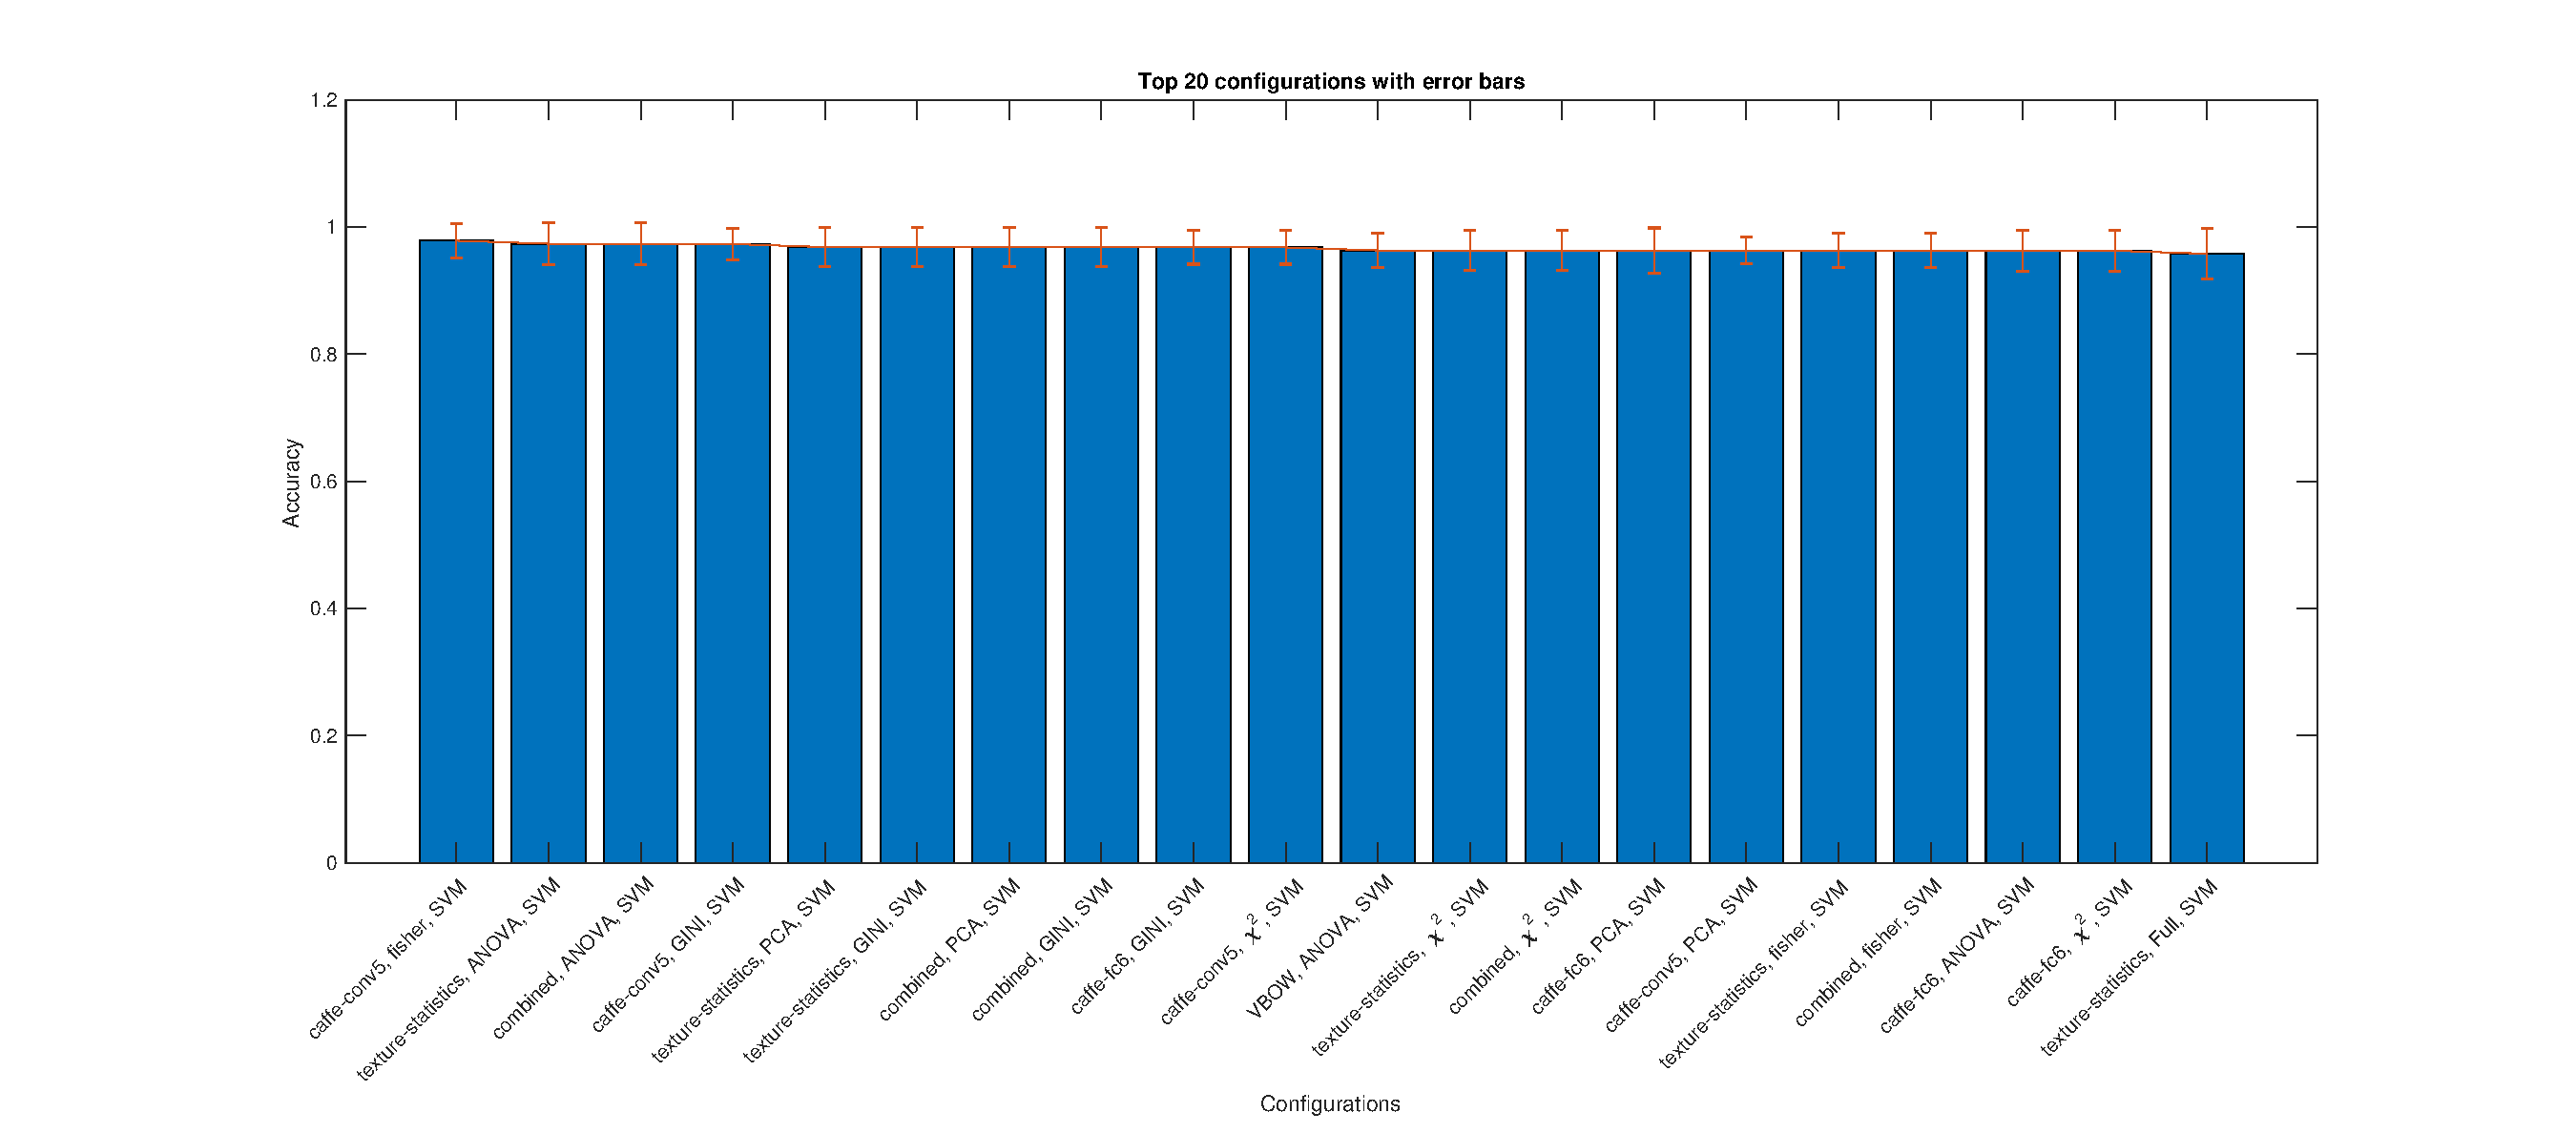
\includegraphics[scale=0.4]{img/best_trans_long_error_bars_20.eps}
 \caption{Top 20 configurations of algorithms in Task 2 with error bars representing one standard deviation. There is no significant difference in the accuracies in the different configuations. Most of the feature extraction algorithms in the top 20 configurations are pre-trained CNNs (\textit{caffe-fc6} or \textit{caffe-conv5})}
 \label{fig:error_bars2}
 \end{centering}
\end{figure}

From the results in Table \ref{table:average_rank2}, we observe that caffe-fc6, PCA and SVM are the highest ranked algorithms. We also note that in this case, the difference in rank between SVM and the next best classification algorithm (NN) is much greater than the corresponding differences in feature extraction and dimensionality reduction. This indicates that the SVM classification algorithm provides superior performance with respect to this task.

\begin{table}[ht!]
\centering
\caption{Average rank of the algorithms in Task 2 with respect to feature extraction, dimensionality reduction and classification. The average rank of an algorithm quantifies it's position in the sorted list of configurations.}
\begin{tabular}{ |c|c| } 
 \hline
 \textbf{Feature extraction} & \textbf{Average rank} \\ 
 \hline
 \textbf{caffe-fc6} & \textbf{47.64}\\
 \hline
texture-statistics & 58.64\\
 \hline
VBOW & 70.5 \\
 \hline
combined & 81.82\\
 \hline
caffe-conv5 & 93.89\\
 \hline
 \hline
 \textbf{Dimensionality reduction} & \textbf{Average rank} \\ 
 \hline
 \textbf{PCA} & \textbf{54.45}\\
 \hline
$\chi^2$ & 58.05\\
\hline
ANOVA & 61.80\\
 \hline
GINI & 66.10\\
 \hline
 fisher & 66.55\\ 
 \hline
Full & 69.6 \\
 \hline
 \hline
 \textbf{Classification} & \textbf{Average rank} \\ 
 \hline
\textbf{SVM} & \textbf{31.22}\\
 \hline
NN & 71.6\\
 \hline
Voting & 75.20 \\
 \hline
RF & 103.97\\
 \hline
 \end{tabular}
\label{table:average_rank2}
\end{table}


\section{Limitations}
\label{limitations}

In this work, pre-trained CNN's were used \cite{Krizhevsky2012}.  Training a convolutional neural network on the small amount of image data provided in Data Sets 1 and 2 (528 and 188 images, respectively) could prove difficult and potentially provide poor results in comparison to the results reported here. The reason for this is that deep neural networks require large image data sets for training because of their capacity to learn complex functions and are therefore prone to overfitting.  The CNN used in this work was previously trained on millions of natural images, allowing for the model to generalize well to new data instances. Even though the original dataset that the neural network was trained on primarily consisted of natural images, we can see (from high classification accuracies) that the features extracted on micrographs provide meaningful representations.

There are an infinite number of potential material microstructures in the realm of materials science.  Micrographs are two-dimensional images that represent a small sample of a three-dimensional microstructure, where `microstructure' refers to material structure on a nanometer to centimeter length scale.  Microstructures are formed from thermodynamic and kinetic processes, and depend on the crystal structure (atomic arrangement) of constituent elements.  Although the elements on the periodic table are fixed, there are numerous combinations of these elements that can be processed and studied. 

Let's first consider a material with a specific chemistry. There are various processes (annealing, quenching, cold working, etc.) that could yield a variety of microstructures.  Additionally, the processed sample could be sectioned in different ways (transverse versus longitudinal, for example), again impacting the microstructure visible for subsequent analysis.  There are also multiple imaging techniques available over a broad range of length scales (nanometer to centimeter).  Images generated from different techniques have different contrast, brightness, and ranges of grayscale intensities or RGB levels.  Expand this thought process to consider all possible material systems that can be generated from known elements with numerous imaging techniques (light optical microscopy, scanning electron microscopy, transmission electron microscopy, etc.).  The possible microstructures we can analyze in the form of image data seems endless.  

Therefore, the variety in micrographs used for materials characterization is vast, which is why expert knowledge and experience is relied on for such tasks as recognition, interpretation, and characterization.  Training an algorithm to perform such classification/characterization tasks on diverse micrograph data sets is a challenge not only in organizing a data set for training, validation, and testing, but in obtaining reasonably good classification results (greater than random).  The limitation presented here, is in the inherent variability of micrograph data, which could make classification tasks challenging, particularly if only a small data set is available for training and testing.  

%----------------------------------------------------------------------------------
\section{Conclusions}
\label{conclusions}

Computer vision and machine learning methods were successfully applied to the challenge of recognizing specific microstructural features of interest (e.g. dendrites) with varying magnifications, chemistries, and orientations.
%
Two binary classification tasks were performed: classification between micrographs with and without dendrites (Task 1), and classification between longitudinal and transverse cross-sectional views of dendrites (Task 2).  Data sets for Task 1 and Task 2 were 528 and 188 total images respectively. We are able to distinguish between microstructural images in terms of the presence of dendrites. A further refinement of the images can also be performed amongst the dendritic micrographs with respect to their cross-section. %The relationship between the two tasks is clearly shown here.
%
\\
Feature extraction and dimensionality reduction techniques were utilized in order to represent micrographs in the form of feature vectors.  Classification was then performed using support vector machines (linear and non-linear), voting, nearest neighbor, and random forest models.
%
For each model, classification accuracy was calculated for full and reduced feature vectors, for each feature extraction and selection method tested. 
\\

Results demonstrated that pre-trained neural networks represented micrographs well, and required no previous knowledge of the nature of shapes or object within the images. Furthermore, when pre-trained neural networks were used in feature extraction the highest classification accuracies for the majority of classifier and feature selection methods tested were achieved. Thus pre-trained neural networks generalize well. 
%
Maximum classification accuracies of 91.85 $\pm$ 4.25\% and 97.37$\pm$ 3.33\% were obtained for Tasks 1 and 2 respectively. 
%
While computer vision and machine learning methods have previously been applied to microstructure image data \cite{DeCost2015, Impoco2015, XuH2015, Bostanabad2016, Taffese2015}, pre-trained deep neural networks have not yet been explored for this particular application, but have proven successful in other image recognition tasks \cite{Guo2016}.  \\

%
Recognition of microstructural features traditionally requires expert knowledge of the particular material system under consideration.  The image-driven machine learning approach to micrograph classification presented here challenges this paradigm. 

This chapter of the Thesis shows how we can use exhaustive grid search based methods to find the best configuration of algorithms and hyperparameters for characterizing microstructures. This method in addition to more methods of hyperparameter optimization like random search, Bayesian optimization and other global optimization methods maybe used to minimize the error from classification tasks in material science and other domains. The next chapter explores the second part of the Thesis, which is to quantify the contributions of different components of an image classification pipeline.


%%----------------------------------------------------------------------------------
%\section{Future Work}
%\label{future_work}
%
%Neural networks are a promising feature extraction method for micrograph representation that could be further developed for application in more sophisticated characterization techniques, thereby eliminating the requirement of expert knowledge for recognition, interpretation, and characterization of microstructrural image data.  
%%
%Future work related to the exploratory study presented here, could involve application of pre-trained CNN's to more diverse micrograph data sets, or higher-level characterization tasks, such as average grain size measurement or calculating area fraction of a second phase.  
%Furthermore, we would also like to incorporate deep learning algorithms on larger and more diverse micrograph classification tasks.
%%----------------------------------------------------------------------------------
%\section*{Acknowledgments}
%\label{acknowledgments}
%This work was is supported by the NSF under Grant \#1056704 through the Metals and Metallic Nanostructures Program of the Division of Materials Research, and Grant \#1302231 through the Information Integration and Informatics Program of the Division of Information and Intelligent Systems.   
%%
%The authors wish to acknowledge Mr. Jesse Werden and Dr. Jie Mao for some of the image data used in this work. 
%%
%Additionally, the authors thank the reviewers for providing thoughtful and thorough comments that contributed to the quality and clarity of the manuscript. 
